\section{Aufbau des Systems}
\subsection{Systembeschreibung}
% Bild für Systembeschreibung
\begin{figure}[htbp]
\centering 
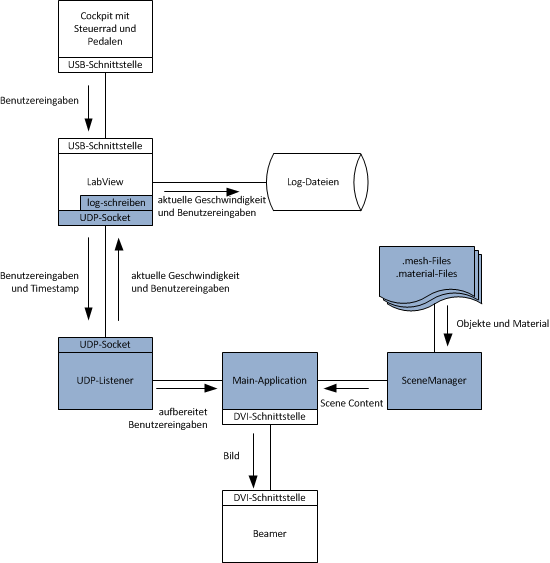
\includegraphics{src/Systembeschreibung.png}
\caption{Systembeschreibung} % Titel der Grafik
\label{Systembeschreibung} % Labelname
\end{figure}

Der Aufbau des Systems für den Fahrsimulator wird anhand der Abbildung \ref{Systembeschreibung} ilustriert. Die blau markierten Komponenten werden im Rahmen dieser Projekt Arbeit entwickelt. Alle übrigen sind bereits vorbestehend. 
Benutzereingaben, die im Cockpit gemacht werden, werden von einem LabView Programm eingelesen. Nun benötigt es einen UDP-Port,  über den verschiedenen Eingaben an das Programm weitergeleitet werden. Es handelt sich hierbei um Werte, die das Drehen des Steuerrades und den Druck auf Gas- oder Bremspedal quantifizieren. Zusätzlich wird der UDP-Port auch für das Empfangen diverser Log-Daten, die von unserem Programm gesendet werden, verwendet. Damit die Empfangenen Daten sauber in ein Log-File geschrieben werden, wird das Lab-View Programm erweitert. 
Weiter  muss in Programmiersprache C einen UDP-Socket mit entsprechendem UDP-Listener implementieren werden, um die Benutzereingaben zu empfangen. Gleichzeitig wird der UDP-Listener dazu verwendet die Geschwindigkeit des Fahrzeugs sowie Timestamps und weitere Daten an das Lab-View Programm zurück zu schicken. Damit können die Daten gespeichert und später ausgewertet werden.
\\
Diese Aufteilung durch eine Netzwerkschnittstelle ermöglicht es,  das System, wenn notwendig, zu dezentralisieren. Einfahheitshalber wurde der UDP-Listener erst in einem Video-Beispiel implementier und getestet (Siehe Anhang B). Nachfolgend wird dieser UDP-Listener auch in das Programm des Fahrsimulator transferiert.
Sind die Daten vom UDP-Listener empfangen und aufbereitet, werden sie im Hauptprogramm (Main Application) weiter verwendet. Während die Position des Steuerrades, des Gas und Bremspedales vom UDP-Listener permanent an das Hauptprogramm übertragen werden, wertet dieses die Positionen aus und veranlass die entspechenden Aktionen in der geladenen Szene. 
Die Szene selbst wird von einem Szenen-Manager geladen. Dieser benötig für die zu ladenden Objekte ein Meshfiles und mindestens ein Materialfile. Die Form jedes Objektes in der Szene wird durch ein separates Meshfile definiert. Texturen und Materialien werden durch ein oder mehrere Materialfiles beschrieben. Ein Materialfile kann zur Beschreibung unterschiedlicher Objekte verwendet werden. Die berechnete Szene wird schlussendlich in einem Fenster von Hauptprogramm angezeigt und über eine DVI-Schnittstelle an den Beamer übertragen. Der Beamer projeziert das Bild an die Wand, die sich direkt vor dem Cockpit befindet. 

\subsection{Anforderungen}
\subsubsection{Funktionale Anforderungen}
Der Fahrsimulator soll eine vordefinierte Szene laden, in der man, durch manipulation am Steuerrad oder der Pedale im Cockpit, das Fahrzeug in der Szene bewegen kann. Die manipulationen des Benutzers solle aufgezeichnet werden um diese auszuwerten. 
\subsubsection {Nicht Funktionale Anforderungen}
\renewcommand{\labelenumi}{\alph{enumi})}
\begin{enumerate}
\item Zuverlässigkeit\\
Die Fahrsimulation soll bei keiner Benutzereingabe die im Cockpit getätigt werden kann, abstürzen oder sich selbts beenden. Zudem sollen alle wichtigen Daten jederzeit in ein log-File geschrieben werden um später Auswertungen vornehmen zu können. 
\item Benutzbarkeit\\
Das Starten des Fahrsimulator sollte möglichst einfach gehalten werden. Das Steuer des Fahrzeuges soll möglichst intuitiev sein wie man es sich von einem richtigen Fahrzeug gewöhnt ist. 
\item Aussehen und Handhabung\\
Der Fahrsimulator soll dem Probanden eine möglichst realistische Fahrsimulation bieten in der sich Strassen und verschiedene Objekte befinden. Die Objekte sollen teilweise aus google-sketchup in das Programm importiert werden um die Simulation noch realistischer zu gestalten. 
\item Zeitliche Anforderungen\\
Die Verzögerungszeit mit der Benutzereingaben und andere Daten wie Geschwindigkeit in das Log-File gespeichert werden, muss kalkuliert werden. Da die Benutzereingaben zweimal über den UDP-Socket müssen (siehe Abbildung \ref{Systembeschreibung}) kann es durchaus zu Verzögerungen kommen. 


Die Verzögerungszeiten die bei Übertragungen von Daten entsehen müssen kalkuliert werden, um spätere Messungen interpretieren zu können. Folgende Verfälschungen sind denkbar bei zu grossen Verögerungszeiten: 
- Der Proband ist irritiert da das Fahrzeug nicht unmittelbar auf seine Eingaben reagiert
- Bei der Auswertung der Daten entsteht der Eindruck der Proband habe zu spät reagiert


\end{enumerate}
